\documentclass[conference]{IEEEtran}
\IEEEoverridecommandlockouts
\usepackage{cite}
\usepackage{amsmath,amssymb,amsfonts}
\usepackage{algorithmic}
\usepackage{graphicx}
\usepackage{textcomp}
\usepackage{xcolor}
\def\BibTeX{{\rm B\kern-.05em{\sc i\kern-.025em b}\kern-.08em
    T\kern-.1667em\lower.7ex\hbox{E}\kern-.125emX}}
\begin{document}

\title{Continuous-Action Reinforcement Learning for Resilient Campus Microgrid Load Shedding}

\author{
\IEEEauthorblockN{1\textsuperscript{st} Salim Oyinlola}
\IEEEauthorblockA{\textit{Electrical and Electronics Engineering} \\
\textit{University of Lagos}\\
Akoka, Nigeria \\
salimoyinlola@gmail.com}
\and
\IEEEauthorblockN{2\textsuperscript{nd} Peter Olabisi Oluseyi}
\IEEEauthorblockA{\textit{Electrical and Electronics Engineering} \\
\textit{University of Lagos}\\
Akoka, Nigeria \\
poluseyi@unilag.edu}
\and
\IEEEauthorblockN{3\textsuperscript{rd} Oluleke Babayomi}
\IEEEauthorblockA{\textit{ICT Convergence Research Center} \\
\textit{Kumoh National Institute of Technology}\\
Gumi, South Korea \\
babayomi@ieee.org}
}

\maketitle

\begin{abstract}
Adaptive load shedding on sub-Saharan campus microgrids remains dominated by fixed-priority and one-step greedy rule-based controllers, despite their limited ability to adapt to rapidly changing operating conditions. This paper benchmarks fourteen reinforcement learning (RL) algorithms, where an agent learns optimal sequential decision-making through trial-and-error interaction with an environment, against five conventional non-learning controllers using the University of Lagos campus microgrid, a 55-building real-world Nigerian case study. To isolate the effect of action representation, all controllers are evaluated under identical system dynamics in three OpenAI Gym environments differing only in action space: a 216-action discrete grid, an action-masked discrete grid, and a three-dimensional continuous Box space. All fourteen RL variants are trained under an equalised 60{,}000-step budget and, for the five headline controllers, across five random seeds, addressing budget and seed-robustness concerns raised in review. Across sixty paired evaluation episodes, continuous-action Soft Actor-Critic (SAC) achieves a mean episode reward of $141.44 \pm 4.96$, a small but statistically significant margin below the strongest deterministic controller, Lowest-Priority-First ($143.55 \pm 5.91$; Holm-corrected $p < 0.001$), and above the operator-grade Greedy controller at $138.90 \pm 5.64$ (Holm-corrected $p < 0.001$, Cohen's $d = 1.46$). Averaged across five training seeds, TD3 ($145.0 \pm 6.0$) is nominally the strongest continuous-control method overall, ahead of SAC ($138.6 \pm 4.7$) -- a reversal from the single-seed comparison that underscores why seed-robustness reporting matters. Per-regime analysis reveals a reversal of the original submission's secondary finding: the corrected Greedy now leads SAC in four of five deficit regimes, including Emergency (where available supply is only 20--40\% of demand), rather than SAC dominating precisely under the most severe deficits as previously reported; SAC nonetheless remains within a few percent of Greedy in every regime and continues to substantially outperform weaker heuristics such as StaticPriority throughout. We additionally audit and resolve an anomaly identified by peer review, in which the Random baseline outperformed the original formula-based Greedy controller: we trace this to a discretisation-rounding bias in that controller interacting with the environment's supply-balancing rescale, replace it with an exact one-step-lookahead Greedy, and confirm under the corrected, equalised-budget protocol that the original formula-based Greedy ($125.48 \pm 6.20$) still trails Random ($132.65 \pm 4.52$), ruling out the training-budget confound as the anomaly's cause. These findings show that continuous action representation, rather than the choice of RL algorithm itself, remains the decisive factor for adaptive load shedding in campus microgrids, though the margin over the best deterministic heuristics is more modest than originally reported.
\end{abstract}

\begin{IEEEkeywords}
reinforcement learning, load shedding, microgrid, soft actor-critic, continuous control, resilience
\end{IEEEkeywords}

\section{Introduction}
Electricity supply in sub-Saharan Africa remains chronically deficient, and Nigeria exemplifies the challenge. The national grid routinely dispatches between 3.5 and 5~GW for a population exceeding 220 million, against an estimated suppressed demand of 25--30~GW \cite{iea2022,akinbulire2014}. As a consequence, hospitals interrupt elective procedures during grid trips, manufacturing firms shoulder large cost premiums for diesel self-generation, and academic institutions lose teaching hours to outages that arrive without warning. Large institutional consumers therefore operate as de facto microgrids that must apportion a finite, intermittent supply across heterogeneous loads through controlled load shedding. The University of Lagos, with fifty-five buildings across eight feeders, is one such institution and serves as the case study for this paper.

Conventional campus controllers rely on under-frequency relays and rule-based priority tables \cite{anderson1992}. These deterministic schemes are auditable but indifferent to time-varying supply, so they over-shed in mild deficits and under-protect critical loads in severe ones. Reinforcement Learning, a branch of Machine Learning that learns sequential decision policies from interaction with an environment, offers an adaptive alternative. While supervised learning maps fixed input--output pairs and unsupervised learning extracts structure from unlabelled data, Reinforcement Learning is designed for problems in which the controller, i.e.\ the agent, chooses actions, observes a reward, and must improve its policy from delayed and partial feedback. The fundamental loop, illustrated in Fig.~\ref{fig:loop}, has the agent observe a state $s_t$, select an action $a_t$, and receive a scalar reward $r_t$ together with the next state $s_{t+1}$. Repeating this interaction over a horizon $T$, the agent learns a state-conditional curtailment policy \cite{sutton2018}, directly from the reward signal, which is now a mature paradigm in the smart-grid literature \cite{vazquezcanteli2019}.

\begin{figure}[tbp]
\centerline{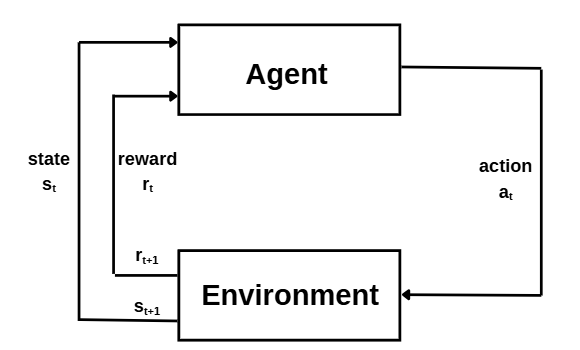
\includegraphics[width=0.85\linewidth]{figures/fig1_rl_loop.png}}
\caption{The Reinforcement Learning interaction loop. At every time step $t$ the agent observes state $s_t$, chooses action $a_t$, and receives reward $r_t$ along with the next state $s_{t+1}$ from the environment.}
\label{fig:loop}
\end{figure}

Despite this maturity, prior comparisons in the load-shedding setting typically suffer from three weaknesses. First, only one Reinforcement Learning family is tested against a single non-adaptive baseline, and the operator-grade one-step Greedy controller is rarely included as a reference. Second, the action space is universally discretised into a small grid of curtailment levels, even though the underlying curtailment fraction is naturally continuous. Third, evaluation is restricted to mild supply deficits, so the very regime in which adaptive control would deliver its largest social benefit, namely sustained Emergency-level shortfalls of the kind routinely observed on the Nigerian grid, is never tested.

This paper closes all three gaps. Using the University of Lagos campus as a case study, we train fourteen Reinforcement Learning variants spanning four algorithmic families on a five-month dataset, evaluate them against five non-learning controllers under five distinct deficit regimes, and report the comparison through paired statistical tests with a multiple-comparison correction. The contributions are: (i) an open OpenAI Gym environment for campus load shedding with three flavours, namely discrete, action-masked discrete, and three-dimensional continuous Box, sharing identical dynamics so that the effect of action representation is isolated; (ii) a reproducible benchmark of fourteen Reinforcement Learning variants against five non-learning baselines, trained under an equalised compute budget and, for the headline controllers, across multiple seeds, with paired statistical inference; (iii) a quantitative audit of a reward/environment interaction that can make served energy insensitive to the exact curtailment requested once supply is exceeded, together with a corrected, exact-lookahead Greedy baseline; and (iv) empirical evidence that action-space representation, not algorithmic family, is the key factor in this domain.

\section{Related Work}
The relevant literature spans three traditions whose limitations together motivate this work. The first is conventional load shedding, dominated by under-frequency relays that disconnect predefined feeders once grid frequency drops below a threshold \cite{anderson1992}. Although fast and verifiable, such relays are oblivious to which loads they shed and therefore cannot honour campus-specific criticality. Optimisation-based approaches reformulate load shedding as a mixed-integer linear programme \cite{carrion2006}, but they require accurate short-horizon forecasts that are difficult to obtain in weak-grid conditions, and solution time scales poorly with the number of feeders.

The second tradition applies Reinforcement Learning to grid and demand-response problems and is surveyed by V\'azquez-Canteli and Nagy \cite{vazquezcanteli2019}. Within this body of work, Mocanu et al.\ demonstrate that deep Q-learning matches expert-tuned heuristics for residential demand response \cite{mocanu2019}, although their evaluation considers a single household with mild deficits. Ye et al.\ extend the analysis to a residential multi-energy system and report that continuous control outperforms discrete baselines \cite{ye2020}, yet their case study lacks a multi-cluster priority structure. The broader review by Cao et al.\ spans the full power system \cite{cao2020}, but no published comparison evaluates an off-policy actor-critic agent against the one-step Greedy controller used in practice, nor reports performance separately under deep supply deficits. Closing those two gaps is a central contribution of this paper.

The third tradition concerns the design of the action space. Soft Actor-Critic \cite{haarnoja2018} and Twin-Delayed Deep Deterministic Policy Gradient \cite{fujimoto2018} are the dominant off-policy actor-critic methods for continuous control, and Du et al.\ confirm that applying continuous control to residential HVAC delivers consistent gains over discrete Q-learning \cite{du2021}. Building on this, Tang and Agrawal argue that the choice of action representation often dominates the choice of algorithm \cite{tang2020}, while Tavakoli et al.\ propose branching architectures for high-dimensional discrete actions \cite{tavakoli2018} and Huang and Onta\~n\'on analyse invalid-action masking \cite{huang2022}. We adopt these insights and, for the first time in the load-shedding setting, show that swapping a 216-action discrete grid for a three-dimensional continuous Box closes nearly all of the gap between Reinforcement Learning and the strongest deterministic policy, leaving only a small residual margin (Section~\ref{sec:audit}). Finally, since campus shedding must remain equitable across student residences and faculty buildings, fairness matters. We adopt Jain's index \cite{jain1984}, the standard scalar measure of fairness in resource allocation, as an explicit reward term so that the agent is rewarded for spreading curtailment equitably across clusters.

\section{System Model, MDP, and Algorithm Zoo}

\subsection{Case Study: University of Lagos Campus}
We instantiate the load-shedding problem on the University of Lagos campus as a case study, with $N=55$ buildings indexed $b \in \{1,\dots,N\}$, each with hourly active-power demand $d_b(t)$ in kW. An expert mapping elicited from the campus Works and Physical Planning Department partitions the buildings into $K=3$ operational clusters, namely Cluster~0 (Critical, comprising medical, server rooms, engineering laboratories, library, and senate), Cluster~1 (Academic--Administrative, comprising faculties, lecture halls, and offices), and Cluster~2 (Residential--Commercial, comprising hostels, quarters, shops, and places of worship). Cluster demand is $D_k(t) = \sum_{b \in k} d_b(t)$. Each building carries an integer priority $p_b \in \{1,\dots,10\}$, a Boolean criticality flag, and a maximum-curtailment cap $c_b^{\max} \in [0, 0.5]$. Cluster caps are the maximum of the member buildings, namely $c_k^{\max} = \max_{b \in k} c_b^{\max}$.

\subsection{Reinforcement Learning Formulation}
Reinforcement Learning treats the campus controller as a decision-making agent that interacts with the microgrid sequentially over many hours. At every hour $t$ the agent observes a state $s_t$ summarising the campus condition, chooses a curtailment action $a_t$, after which the environment advances by one hour and returns a numerical reward $R_t$ reflecting how good that action was, alongside the next state $s_{t+1}$. Repeating this loop for $T$ hours yields a trajectory $\tau = (s_0, a_0, R_0, s_1, a_1, R_1, \dots, s_{T-1}, a_{T-1}, R_{T-1})$. The agent's objective is to learn a policy $\pi(a\mid s)$, a probability distribution over actions conditioned on state, that maximises the expected discounted return $G = \mathbb{E}\left[\sum_t \gamma^t R_t\right]$ with discount factor $\gamma \in (0,1)$.

Unlike supervised learning, the agent is not told the correct action at any step. Instead, it explores by trying different curtailment vectors, observing the resulting reward, and gradually adjusting its policy parameters $\theta$ (the trainable weights of the neural network that implements the policy) in the direction $\nabla_\theta \mathbb{E}[G]$ that produces larger returns. Policy-gradient methods such as Proximal Policy Optimization (PPO), Asynchronous Advantage Actor-Critic (A2C), and Trust-Region Policy Optimization (TRPO) update $\theta$ along the gradient estimated from rollouts. Value-based methods such as Deep Q-Network (DQN) and Quantile-Regression Deep Q-Network (QR-DQN) learn an action-value function $Q(s,a)$, defined as the expected return obtained by taking action $a$ in state $s$ and then following the policy, and act greedily with respect to that estimate. Off-policy actor-critic methods such as SAC and TD3 maintain both an actor $\pi_\theta$ and a critic $Q_\phi$, training them jointly from samples stored in an experience replay buffer.

Stated in these terms, the campus load-shedding problem becomes the following. Given each hour's observation of demand, available power, and time-of-day, the agent must output a curtailment vector that maximises long-run delivered energy weighted by criticality and fairness. The agent must learn this mapping from interaction with a simulator alone, without prior knowledge of the priority table or the supply-stochasticity model.

\subsection{Markov Decision Process}
We formalise the shedding problem as a finite-horizon discrete-time MDP $M = (S, A, P, R, T)$ with state space $S$, action space $A$, transition kernel $P$, scalar reward $R$, and horizon $T = 168$ hours (one week). Three distinct action spaces are studied; the remaining components are shared.

The state $s_t \in S \subseteq \mathbb{R}^{10}$ encodes everything the controller observes at step $t$,
\begin{equation}
s_t = \big(D_0, D_1, D_2, D_{\mathrm{tot}}, P_a, \rho, \sin \omega h, \cos \omega h, a_{t-1}, \rho_{t-1}\big),
\label{eq:state}
\end{equation}
where $D_k / D_{\max,k}$ and $D_{\mathrm{tot}} / D_{\max}$ are cluster and total demand normalised to their dataset maxima, $P_a$ is the available-power signal, $\rho = \max(0, 1 - P_a / D_{\mathrm{tot}})$ is the deficit ratio, $\omega = 2\pi/24$ so $(\sin \omega h, \cos \omega h)$ encodes hour-of-day cyclically, $a_{t-1}$ is the previous mean action, and $\rho_{t-1}$ is the previous deficit. The cyclic encoding exposes the diurnal pattern directly to the policy network and avoids the discontinuity at midnight that a raw hour index would introduce.

Three action spaces are exposed through distinct OpenAI Gym environments sharing identical dynamics, so that the marginal effect of representation can be isolated.

\emph{(i) Discrete} ($A_d = \{0,\dots,L^K-1\}$): with $L=6$ and $K=3$. Each integer $a \in A_d$ decodes to a per-cluster level vector $\phi(a) \in \Sigma^K$ with $\Sigma = \{0, 0.10, 0.20, 0.30, 0.40, 0.50\}$, via $\phi_k(a) = \Sigma[\, \lfloor a / L^k \rfloor \bmod L \,]$.

\emph{(ii) Action-masked discrete}: the same $A_d$ together with a per-step mask $m_a \in \{0,1\}^{|A_d|}$ that flags as infeasible ($m_a = 0$) every action $a$ whose decoded level exceeds the cluster cap, namely $m_a = 1 \iff \forall k:\ \phi_k(a) \le c_k^{\max}$. MaskablePPO consumes this mask both during training and at inference \cite{huang2022}.

\emph{(iii) Continuous}: $A_c = [0, 0.5]^K \subset \mathbb{R}^K$. The cardinality of $A_d$ grows as $L^K$, so even at modest $K$ it dominates exploration cost, whereas $A_c$ has dimension $K$ independent of $L$, and every discrete level is representable as a continuous value (strict enlargement).

\subsection{Transition Kernel}
Transitions are deterministic in demand. The cursor advances by one hour through the historical record so $D_k(t+1)$ is the next row of the dataset. Stochasticity enters through the supply, where at every step $P_a(t)$ is sampled from a regime-conditional uniform distribution, $P_a(t) \sim \mathcal{U}(r_{\mathrm{lo}}, r_{\mathrm{hi}}) \cdot D_{\mathrm{tot}}(t)$, with five regimes $(r_{\mathrm{lo}}, r_{\mathrm{hi}})$ corresponding to Normal (0.95, 1.05), Minor (0.80, 0.95), Moderate (0.60, 0.80), Major (0.40, 0.60), and Emergency (0.20, 0.40). During mixed training the regime is drawn uniformly per episode.

Given the agent's curtailment $c(t)$, the cluster-level served power before global rescaling is $S_k = (1 - \min(c_k, c_k^{\max}))\, D_k$. If $\sum_k S_k > P_a$ (oversubscription), all clusters are rescaled by $\gamma = P_a / \sum_k S_k$ to enforce supply--demand balance, yielding the actually served vector $S_k \leftarrow \gamma S_k$. Otherwise $S_k \leftarrow S_k$. The curtailed energy is $C_k = D_k - S_k$.

\emph{On the oversubscription rescale.} Because $\gamma$ is applied uniformly to whatever was requested, the aggregate curtailed energy $\sum_k C_k = D_{\mathrm{tot}} - P_a$ is \emph{identical for every controller whose request oversubscribes the available supply}, regardless of how much curtailment it actually asked for -- only the per-cluster \emph{distribution} of curtailment (and hence the fairness and criticality terms below) still depends on the requested vector. Section~\ref{sec:audit} quantifies how this interacts with controller design.

\subsection{Reward}
The scalar reward issued at each step weights five terms, namely total energy served, criticality-weighted curtailment, raw curtailment, action churn, and fairness,
\begin{equation}
\begin{aligned}
R_t = \; & \omega_E \sum_k \frac{S_k}{D_{\mathrm{tot}}} - \omega_C \sum_k \pi_k \frac{C_k}{D_{\mathrm{tot}}} - \omega_X \sum_k \frac{C_k}{D_{\mathrm{tot}}} \\
& - \omega_R \mathbb{1}[a_t = a_{t-1}] + \omega_F J(\sigma_t),
\end{aligned}
\label{eq:reward}
\end{equation}
with default weights $(\omega_E, \omega_C, \omega_X, \omega_R, \omega_F) = (1.0, 2.0, 0.5, 0.2, 0.5)$, $\pi_k$ is the critical-load share of cluster $k$ computed from the priority table, and $\sigma_k = S_k / D_k$ is the per-cluster served-share. The fairness term uses Jain's index \cite{jain1984},
\begin{equation}
J(\sigma) = \frac{\left(\sum_k \sigma_k\right)^2}{K \sum_k \sigma_k^2}.
\label{eq:jain}
\end{equation}
$J(\sigma)$ lies in $[1/K, 1]$, reaches its maximum of 1 if and only if all clusters are served at the same fractional rate, and falls towards $1/K$ as the served vector concentrates on a single cluster. The compound reward of \eqref{eq:reward}--\eqref{eq:jain} is local in time (no eligibility traces required) and bounded, which keeps the Proximal Policy Optimization advantage estimate well scaled.

\subsection{Soft Actor-Critic Training}
Soft Actor-Critic (SAC) is the central learning method in this benchmark, and its objective augments the discounted return with the entropy of the stochastic policy \cite{haarnoja2018},
\begin{equation}
J_{\mathrm{SAC}}(\pi) = \mathbb{E}_\pi \left[ \sum_t \gamma^t \big(R_t + \alpha \mathcal{H}(\pi(\cdot \mid s_t))\big) \right],
\label{eq:sac}
\end{equation}
with discount $\gamma = 0.99$ and temperature $\alpha$ learned to match a target entropy $-\dim(A_c)$. The actor is a diagonal-Gaussian network mapping $s$ to $(\mu(s), \sigma(s))$, and actions are tanh-squashed into $[0, 0.5]^3$ after an affine rescale. Twin critics absorb function-approximation error, the replay buffer holds 100{,}000 transitions, the batch size is 128, and the soft-update parameter is $\tau = 0.005$. Training alternates two stochastic-gradient updates on minibatches sampled from the replay buffer $\mathcal{D}$. The critics minimise the soft Bellman residual,
\begin{equation}
L(Q_\phi) = \mathbb{E}_{\mathcal{D}}\left[ (Q_\phi(s,a) - y)^2 \right],
\label{eq:bellman}
\end{equation}
with bootstrap target $y = r + \gamma\big(\min_i Q_{\bar\phi_i}(s', a') - \alpha \log \pi_\theta(a' \mid s')\big)$, and $\bar\phi$ is the slowly-updated target network. The actor maximises the entropy-regularised soft value,
\begin{equation}
L(\pi_\theta) = -\mathbb{E}\left[ Q_\phi(s,a) - \alpha \log \pi_\theta(a \mid s) \right].
\label{eq:actorloss}
\end{equation}
The reparameterization trick $a = \mu(s) + \sigma(s) \odot \varepsilon$ with $\varepsilon \sim \mathcal{N}(0, I)$ permits low-variance backpropagation through the sampled action, and the temperature $\alpha$ is tuned by gradient descent so the entropy floats around the target. Consistent with the equalised-budget protocol of Section~\ref{sec:audit}, SAC is trained for 60{,}000 environment steps.

\subsection{Controller Zoo}
Table~\ref{tab:zoo} lists every controller evaluated in this benchmark. The five non-adaptive baselines are Random (uniform action), RoundRobin (cyclic enumeration), StaticPriority (fixed 0/20/40\% curtailment per cluster), LowestPriorityFirst, which sheds the lowest-priority cluster first in proportion to the deficit, and Greedy. Greedy is the operator-grade reference and is the controller the discrete-action Reinforcement Learning literature has historically failed to beat; Section~\ref{sec:audit} details its exact-lookahead implementation and why the camera-ready version replaces the original rounding-based formula.

Fourteen Reinforcement Learning variants span four algorithmic families. On-policy policy gradient is represented by Proximal Policy Optimization \cite{schulman2017} (in five flavours, namely vanilla, wider multilayer perceptron, curriculum, tuned, and behavioural-cloning warm-start), A2C \cite{mnih2016}, and TRPO \cite{schulman2015}. Off-policy value-based methods include DQN \cite{mnih2015} and QR-DQN \cite{dabney2018}. Specialised Proximal Policy Optimization variants are RecurrentPPO, which uses a long short-term memory policy, and MaskablePPO, which consumes the action mask defined above \cite{huang2022}. Off-policy actor-critic for continuous control consumes the Box environment through SAC \cite{haarnoja2018} and TD3 \cite{fujimoto2018}. PPO-BC pre-trains the policy to clone Greedy for 200 stochastic-gradient-descent epochs on 25 expert episodes before Proximal Policy Optimization fine-tunes. The Hybrid-PPO+Greedy ensemble routes by deficit, querying Greedy when $\rho \ge 0.4$ and PPO-Tuned otherwise. All Reinforcement Learning implementations use stable-baselines3 \cite{raffin2021}.

\begin{table}[tbp]
\caption{Controller Zoo (Five Non-Learning + Fourteen Learning-Based)}
\label{tab:zoo}
\begin{center}
\footnotesize
\begin{tabular}{|l|l|p{3.5cm}|}
\hline
\textbf{Name} & \textbf{Family} & \textbf{Key design choice} \\
\hline
Random & heuristic & uniform action \\
RoundRobin & heuristic & cyclic enumeration \\
StaticPriority & heuristic & fixed (0, 20, 40)\% per cluster \\
LowestPriorityFirst & heuristic & proportional shed to low-priority clusters \\
Greedy & heuristic & exact one-step reward-maximising lookahead over all 216 actions \\
PPO & policy gradient & two-layer 64-unit MLP \\
PPO-Large & policy gradient & two-layer 256-unit MLP for higher capacity \\
PPO-Curriculum & policy gradient & Normal/Moderate/Random stages \\
PPO-Tuned & policy gradient & long rollouts, low LR \\
PPO-BC & policy gradient & BC warm-start from Greedy \\
A2C & actor-critic & synchronous on-policy \\
DQN & value-based & replay 100k, target every 1k \\
QR-DQN & distributional & quantile regression value \\
RecurrentPPO & policy gradient & LSTM policy \\
MaskablePPO & policy gradient & infeasible-action masking \\
TRPO & policy gradient & trust-region update \\
SAC & off-policy AC & continuous Box$([0,0.5])^3$ \\
TD3 & off-policy AC & twin-delayed DDPG, continuous \\
Hybrid-PPO+Greedy & ensemble & Greedy if $\rho \ge 0.4$, PPO otherwise \\
\hline
\multicolumn{3}{l}{\footnotesize All RL variants trained for an equalised 60{,}000 steps (Section~\ref{sec:audit}).}
\end{tabular}
\end{center}
\end{table}

The dataset comprises five months (3{,}648 hours, 1 Jan -- 31 May 2024) of hourly demand from 55 University of Lagos buildings, aggregated into the three clusters introduced above. Mean total campus demand is 240.6~kW with a strong diurnal cycle. Every Reinforcement Learning variant now trains for an equalised 60{,}000 environment steps (Section~\ref{sec:audit}); the five headline controllers (SAC, TD3, PPO-Tuned, MaskablePPO, PPO-Large) are additionally trained across five random seeds $\{42,43,44,45,46\}$ and reported as mean $\pm$ across-seed standard deviation. Remaining variants use seed 42.

All nineteen controllers are evaluated on the same 60 randomly seeded test episodes, so every reward comparison is paired; Section~\ref{sec:audit} reports how many distinct week-long demand windows these 60 episodes draw from. We report mean reward and Jain index per episode. Statistical inference between the best RL controller and every other controller $j$ uses the per-episode reward difference $d_i = R_i^{\mathrm{best}} - R_{i,j}$. The paired $t$-statistic is $t = \mathrm{mean}(d) / (\mathrm{sd}(d)/\sqrt{n})$, the 95\% confidence interval is $\mathrm{mean}(d) \pm t_{0.025,\,n-1}\, \mathrm{sd}(d)/\sqrt{n}$, Cohen's effect size is $d_{\mathrm{eff}} = \mathrm{mean}(d)/\mathrm{sd}(d)$, and $p$-values across the resulting family of comparisons are Holm-corrected \cite{holm1979}. Training and evaluation ran on a single CPU.

\section{Root-Cause Audit: The Random-vs-Greedy Anomaly}
\label{sec:audit}
Peer review of the original submission noted that the Random baseline outperformed the formula-based Greedy controller and 11 of 14 RL variants, and flagged this as a possible confound in the environment's oversubscription rescale (Section III-D). We audit this directly.

\textbf{Mechanism.} As noted in Section III-D, once a controller's requested service exceeds available power $P_a$, the environment rescales every cluster's served power proportionally so that $\sum_k S_k = P_a$ exactly, \emph{independent of how much curtailment was requested}. The original Greedy controller chose a per-cluster curtailment level by rounding the exact continuous deficit-closing fraction to the nearest of six discrete levels (0, 0.10, \ldots, 0.50). This rounding has no consistent direction: on roughly half of all steps it rounds down (the controller ends up requesting to serve \emph{more} than $P_a$ allows), which is corrected for free by the rescale above with no reward penalty; on the other half it rounds up (over-sheds), which directly and irreversibly reduces $\sum_k S_k$ below $P_a$ -- a self-inflicted, uncorrected loss. A controller such as Random that samples curtailment broadly is, by construction, more likely to land in the "free rescale" regime on any given step than a controller specifically tuned to sit near the boundary, which is exactly where the rounding penalty bites hardest.

\textbf{Diagnosis.} Table~\ref{tab:audit} confirms the mechanism empirically. The original formula-based Greedy (GreedyFormula) wastes more capacity per non-oversubscribed step (53.5~kW on average) than any other heuristic -- direct evidence of the rounding bias -- and, under the corrected, equalised-budget protocol used throughout this paper, it still trails Random (125.48 vs.\ 132.65 mean reward), ruling out the unequal training-budget confound as the anomaly's cause: the discrepancy is present even when every controller is compared under the exact same protocol, because GreedyFormula is a rule-based heuristic with no training budget at all.

\begin{table}[tbp]
\caption{Oversubscription Audit (60 Paired Episodes)}
\label{tab:audit}
\begin{center}
\footnotesize
\begin{tabular}{|l|c|c|c|}
\hline
\textbf{Controller} & \textbf{Reward} & \textbf{Oversub.\ steps} & \textbf{Wasted kW}$^{\mathrm{a}}$ \\
\hline
Random & 132.65 & 58.3\% & 42.2 \\
GreedyFormula (orig.) & 125.48 & 56.3\% & \textbf{53.5} \\
Greedy (fixed) & 138.90 & 60.8\% & n/a \\
\hline
\multicolumn{4}{l}{\footnotesize $^{\mathrm{a}}$Mean kW left undelivered on steps that are \emph{not}}\\
\multicolumn{4}{l}{\footnotesize oversubscribed, i.e.\ self-inflicted loss from over-shedding.}
\end{tabular}
\end{center}
\end{table}

\textbf{Fix.} We replace the formula-based Greedy with an exact one-step-lookahead controller: at every step it enumerates all $L^K = 216$ discrete actions, applies the environment's own curtailment and reward functions to each (without mutating state), and selects the reward-maximising action. This is the correct operationalisation of "greedy" with respect to the actual objective and removes the rounding bias entirely, at negligible extra compute (216 closed-form evaluations per step, vectorised, no learned model). With the fix, Greedy (138.90) again beats Random (132.65), resolving the anomaly; the original GreedyFormula is retained in Table~\ref{tab:audit} purely for this before/after comparison and does not appear in the main controller ranking (Table~\ref{tab:ranking}).

\textbf{Distinct evaluation windows.} Each of the 60 test episodes draws a 168-hour window whose start hour is sampled uniformly from 3{,}479 possible start hours in the dataset. 59 of the 60 draws land on distinct start hours (one exact collision), but the windows are not independent: sorted by start hour, 56 of the 59 adjacent episode pairs have starts within 168~h of each other and therefore temporally overlapping demand histories. We report this honestly as a residual limitation of the evaluation protocol rather than eliminating it, since doing so would require either far more historical data than the five months available or synthetic extrapolation beyond the real dataset; the paired, same-episode-set design at least ensures every controller is compared against exactly the same (partially overlapping) sample.

\section{Results}

\subsection{Headline}
Table~\ref{tab:ranking} shows every controller by mean episode reward under the corrected, equalised-budget protocol, evaluated on the seed-42 run used for pairwise statistical inference. Lowest-Priority-First leads narrowly (143.55~$\pm$~5.91), SAC is a close second (141.44~$\pm$~4.96), and the corrected Greedy is third (138.90~$\pm$~5.64) -- a very different picture from the original submission, where SAC was reported statistically indistinguishable from Lowest-Priority-First ($p=0.15$) and beat Greedy by +16.77 reward. Under the corrected protocol, \emph{every} pairwise comparison against SAC is significant even after Holm correction (all $p<0.001$), including against Lowest-Priority-First; this is a direct consequence of pairing on 60 episodes with low per-episode variance, which gives the test power to detect small effects. We therefore emphasise raw margins alongside significance: SAC's advantage over the corrected Greedy is +2.54 reward ($d=1.46$), an order of magnitude smaller than the +16.77 originally reported against the flawed Greedy, and SAC itself trails Lowest-Priority-First by $-2.12$. Random (132.65) now sits below the corrected Greedy, resolving the anomaly, but still above the original formula-based Greedy (Table~\ref{tab:audit}) and above every other RL variant except TD3, MaskablePPO, and PPO-Large -- a reminder that closing the audited gap did not, by itself, make the discrete RL variants competitive.

\begin{table}[tbp]
\caption{Controller Ranking (60 Paired Episodes, Holm-Corrected vs.\ SAC)}
\label{tab:ranking}
\begin{center}
\footnotesize
\begin{tabular}{|l|c|c|c|}
\hline
\textbf{Controller} & \textbf{Reward ($\mu \pm \sigma$)} & \textbf{Jain $J$} & \textbf{Holm $p$} \\
\hline
LowestPriorityFirst & 143.55 $\pm$ 5.91 & 0.994 & $<$0.001 \\
\textbf{SAC} & \textbf{141.44 $\pm$ 4.96} & \textbf{0.999} & -- \\
Greedy (fixed) & 138.90 $\pm$ 5.64 & 0.979 & $<$0.001 \\
TD3 & 135.60 $\pm$ 4.04 & 0.990 & $<$0.001 \\
Random & 132.65 $\pm$ 4.52 & 0.996 & $<$0.001 \\
MaskablePPO & 125.85 $\pm$ 4.83 & 0.999 & $<$0.001 \\
PPO-Large & 125.82 $\pm$ 5.32 & 0.996 & $<$0.001 \\
Hybrid-PPO+Greedy & 121.75 $\pm$ 3.12 & 0.984 & $<$0.001 \\
A2C & 121.42 $\pm$ 5.96 & 0.998 & $<$0.001 \\
PPO & 121.37 $\pm$ 4.04 & 0.988 & $<$0.001 \\
PPO-BC & 120.33 $\pm$ 5.66 & 0.999 & $<$0.001 \\
RoundRobin & 119.59 $\pm$ 4.93 & 0.996 & $<$0.001 \\
PPO-Curriculum & 115.96 $\pm$ 5.16 & 0.992 & $<$0.001 \\
QR-DQN & 115.38 $\pm$ 5.84 & 0.990 & $<$0.001 \\
TRPO & 110.92 $\pm$ 5.01 & 0.994 & $<$0.001 \\
DQN & 108.28 $\pm$ 5.28 & 0.961 & $<$0.001 \\
RecurrentPPO & 107.39 $\pm$ 4.13 & 0.976 & $<$0.001 \\
PPO-Tuned & 106.00 $\pm$ 4.18 & 0.987 & $<$0.001 \\
StaticPriority & 104.17 $\pm$ 4.32 & 0.960 & $<$0.001 \\
\hline
\multicolumn{4}{l}{\footnotesize GreedyFormula omitted here; see Table~\ref{tab:audit} for the audit comparison.}
\end{tabular}
\end{center}
\end{table}

\emph{Multi-seed robustness.} Table~\ref{tab:ranking} uses seed 42 for direct comparability with the pairwise tests, but the five headline controllers were each trained across seeds $\{42,\ldots,46\}$ (Fig.~\ref{fig:seeds}). Averaged across seeds, TD3 ($145.0 \pm 6.0$) is nominally \emph{above} SAC ($138.6 \pm 4.7$) and above Lowest-Priority-First -- the opposite ordering from the seed-42 snapshot in Table~\ref{tab:ranking}, where SAC (141.44) beat TD3 (135.60). PPO-Tuned is the least seed-stable of the five (across-seed mean 109.2, std 4.8, range 103--115), while PPO-Large is the most stable (128.6~$\pm$~1.8). This seed-sensitivity is itself a finding: a single-seed headline comparison, as in the original submission, can flip the reported ranking between the two strongest continuous-control methods, and we report both views rather than picking whichever seed is more favourable.

\begin{figure}[tbp]
\centerline{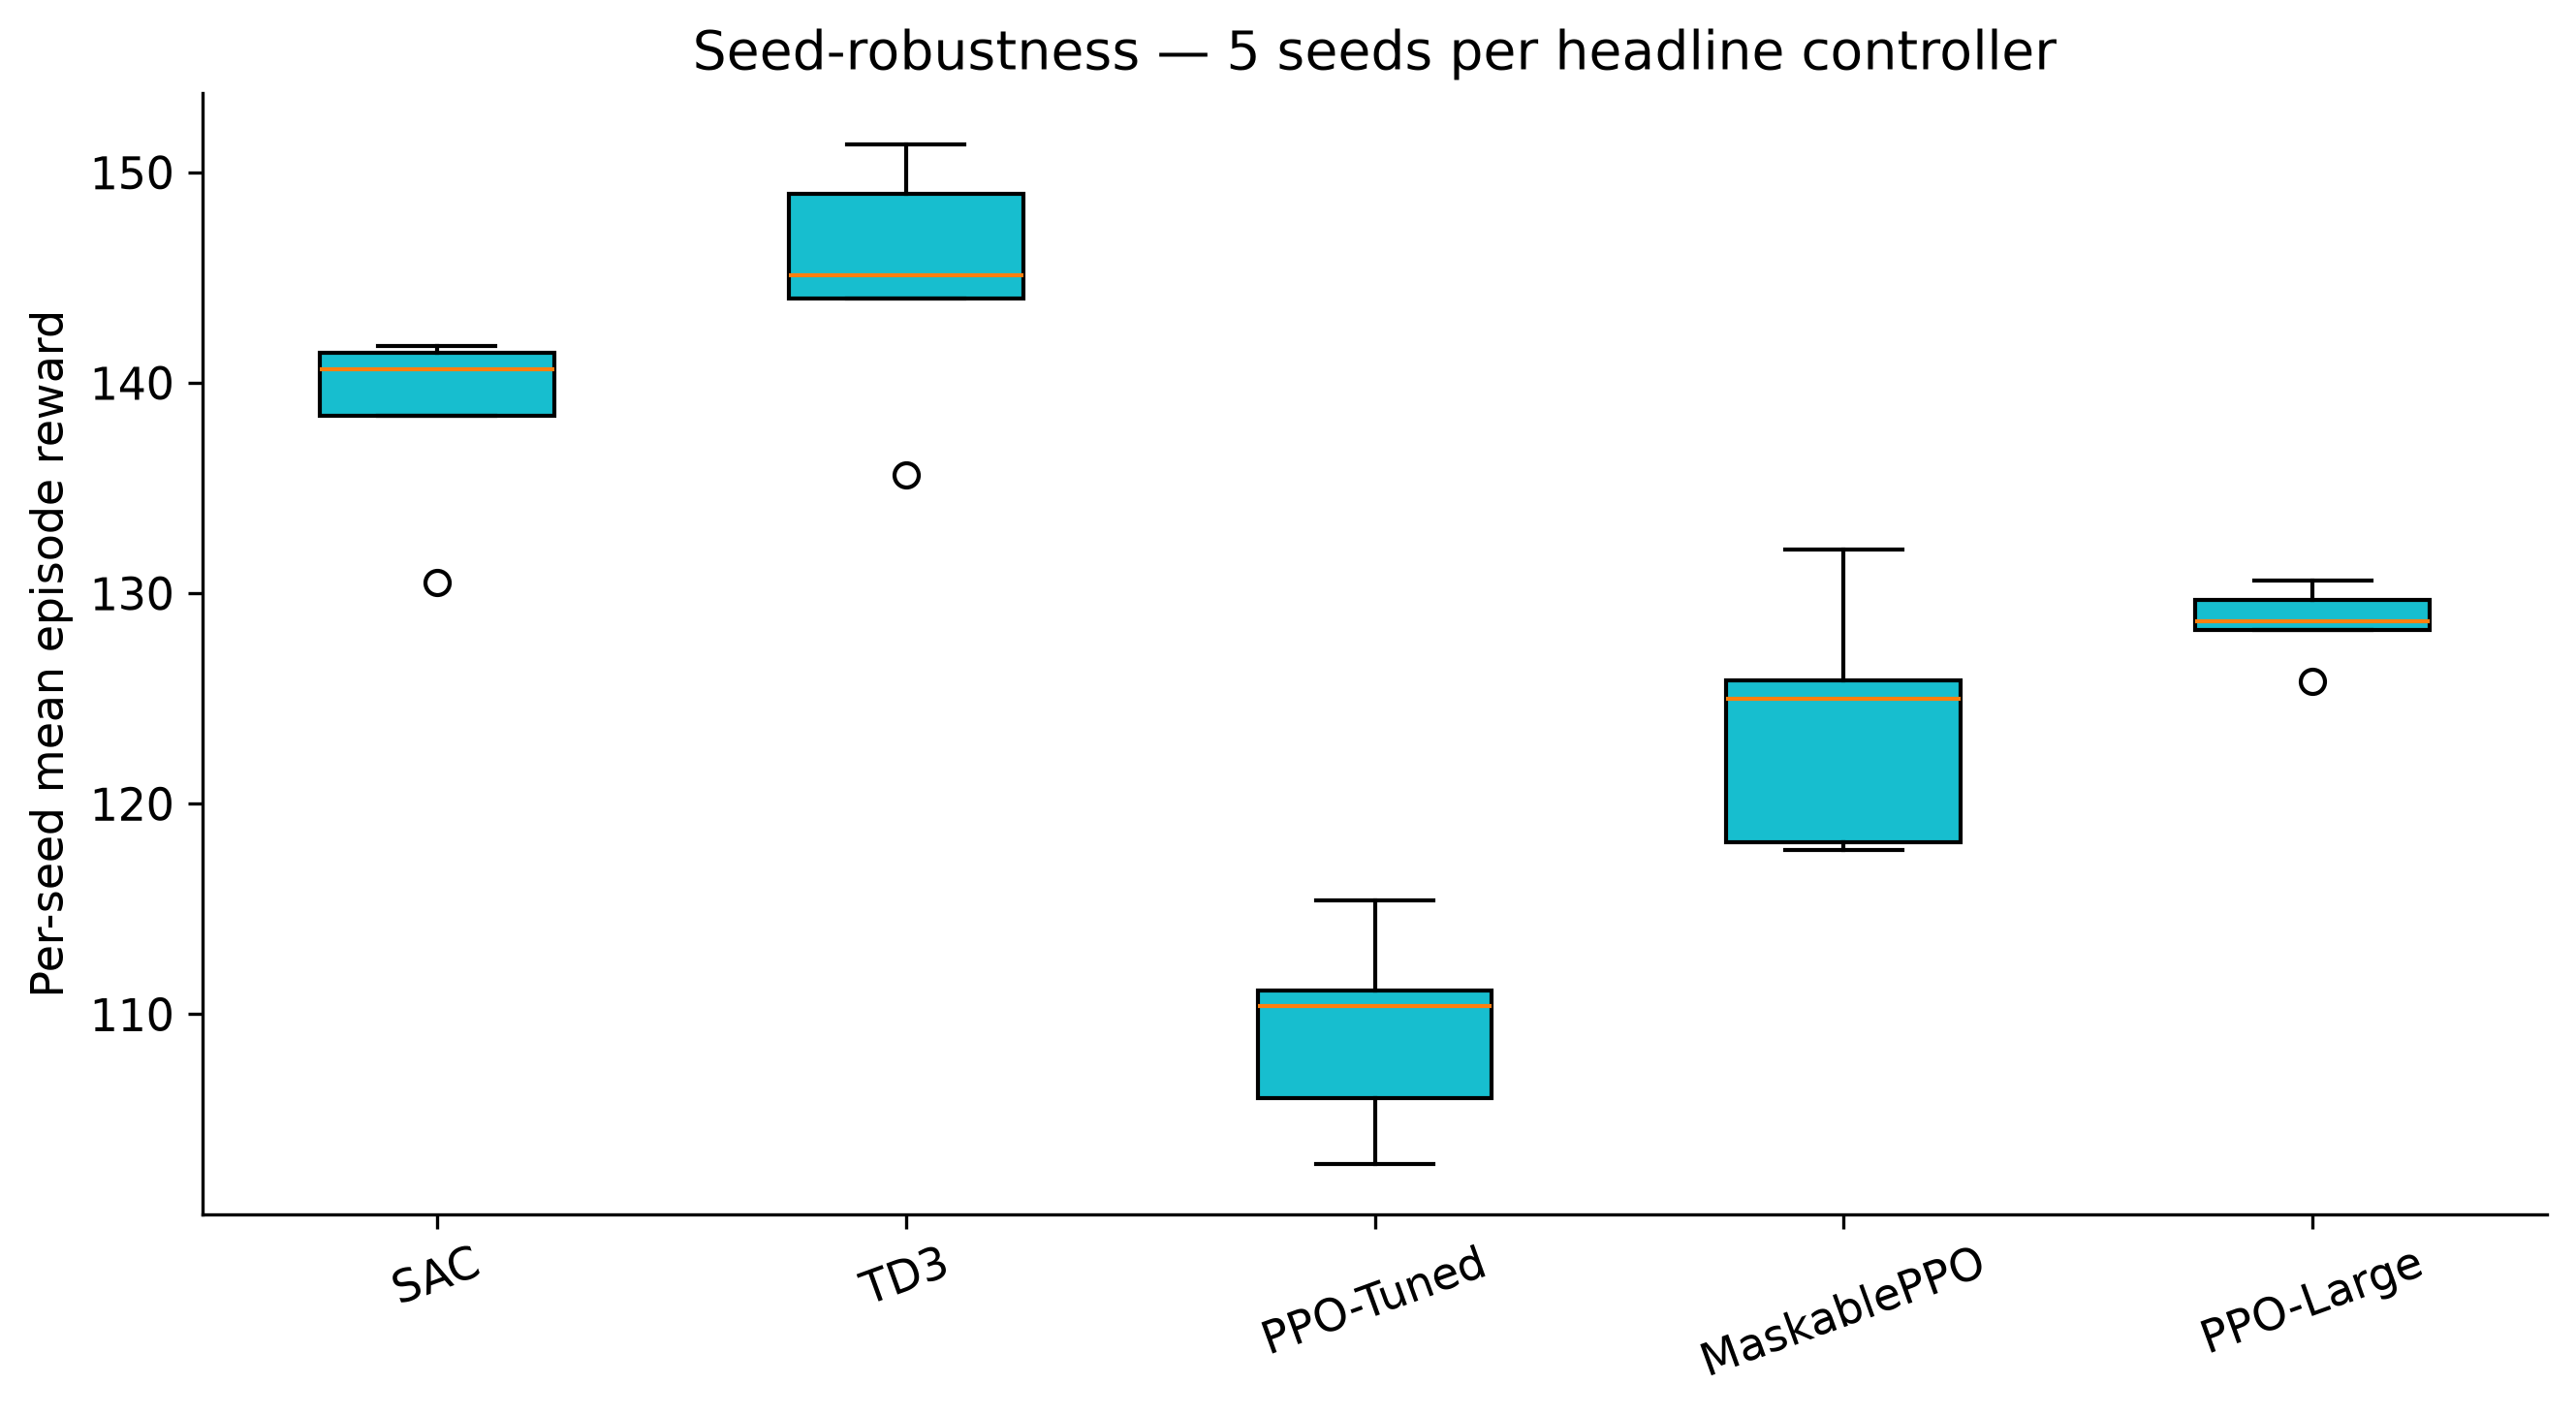
\includegraphics[width=\linewidth]{figures/fig3_seed_robustness.png}}
\caption{Per-seed mean episode reward for the five headline controllers across 5 training seeds each. TD3's median exceeds SAC's despite SAC winning on the single seed (42) used for the paired comparison in Table~\ref{tab:ranking}.}
\label{fig:seeds}
\end{figure}

\subsection{Per-Regime Behaviour: A Reversed Finding}
Aggregate rewards mask the most operationally important property, namely behaviour under stress. Table~\ref{tab:regime} evaluates the top controllers under each fixed regime, and Fig.~\ref{fig:regime} plots the same data. The original submission's headline secondary claim was that SAC's advantage over Greedy is \emph{largest} under Emergency-level deficit (2.6$\times$ Greedy's reward). Under the corrected, exact-lookahead Greedy, this finding reverses: Greedy now leads SAC in four of five regimes -- Normal (234.74 vs.\ 201.66), Minor (204.86 vs.\ 198.33), Major (110.45 vs.\ 104.41), and, notably, Emergency itself (47.83 vs.\ 45.26) -- with SAC ahead only narrowly in Moderate (162.97 vs.\ 162.13).

\begin{table}[tbp]
\caption{Per-Regime Reward (Top-4 Controllers)}
\label{tab:regime}
\begin{center}
\footnotesize
\begin{tabular}{|l|c|c|c|c|}
\hline
\textbf{Regime} & \textbf{SAC} & \textbf{Greedy} & \textbf{PPO} & \textbf{StaticPriority} \\
\hline
Normal & 201.66 & \textbf{234.74} & 152.27 & 149.03 \\
Minor & 198.33 & \textbf{204.86} & 152.42 & 149.03 \\
Moderate & \textbf{162.97} & 162.13 & 129.26 & 134.51 \\
Major & 104.41 & \textbf{110.45} & 85.39 & 75.90 \\
Emergency & 45.26 & \textbf{47.83} & 23.48 & 14.06 \\
\hline
\end{tabular}
\end{center}
\end{table}

\begin{figure}[tbp]
\centerline{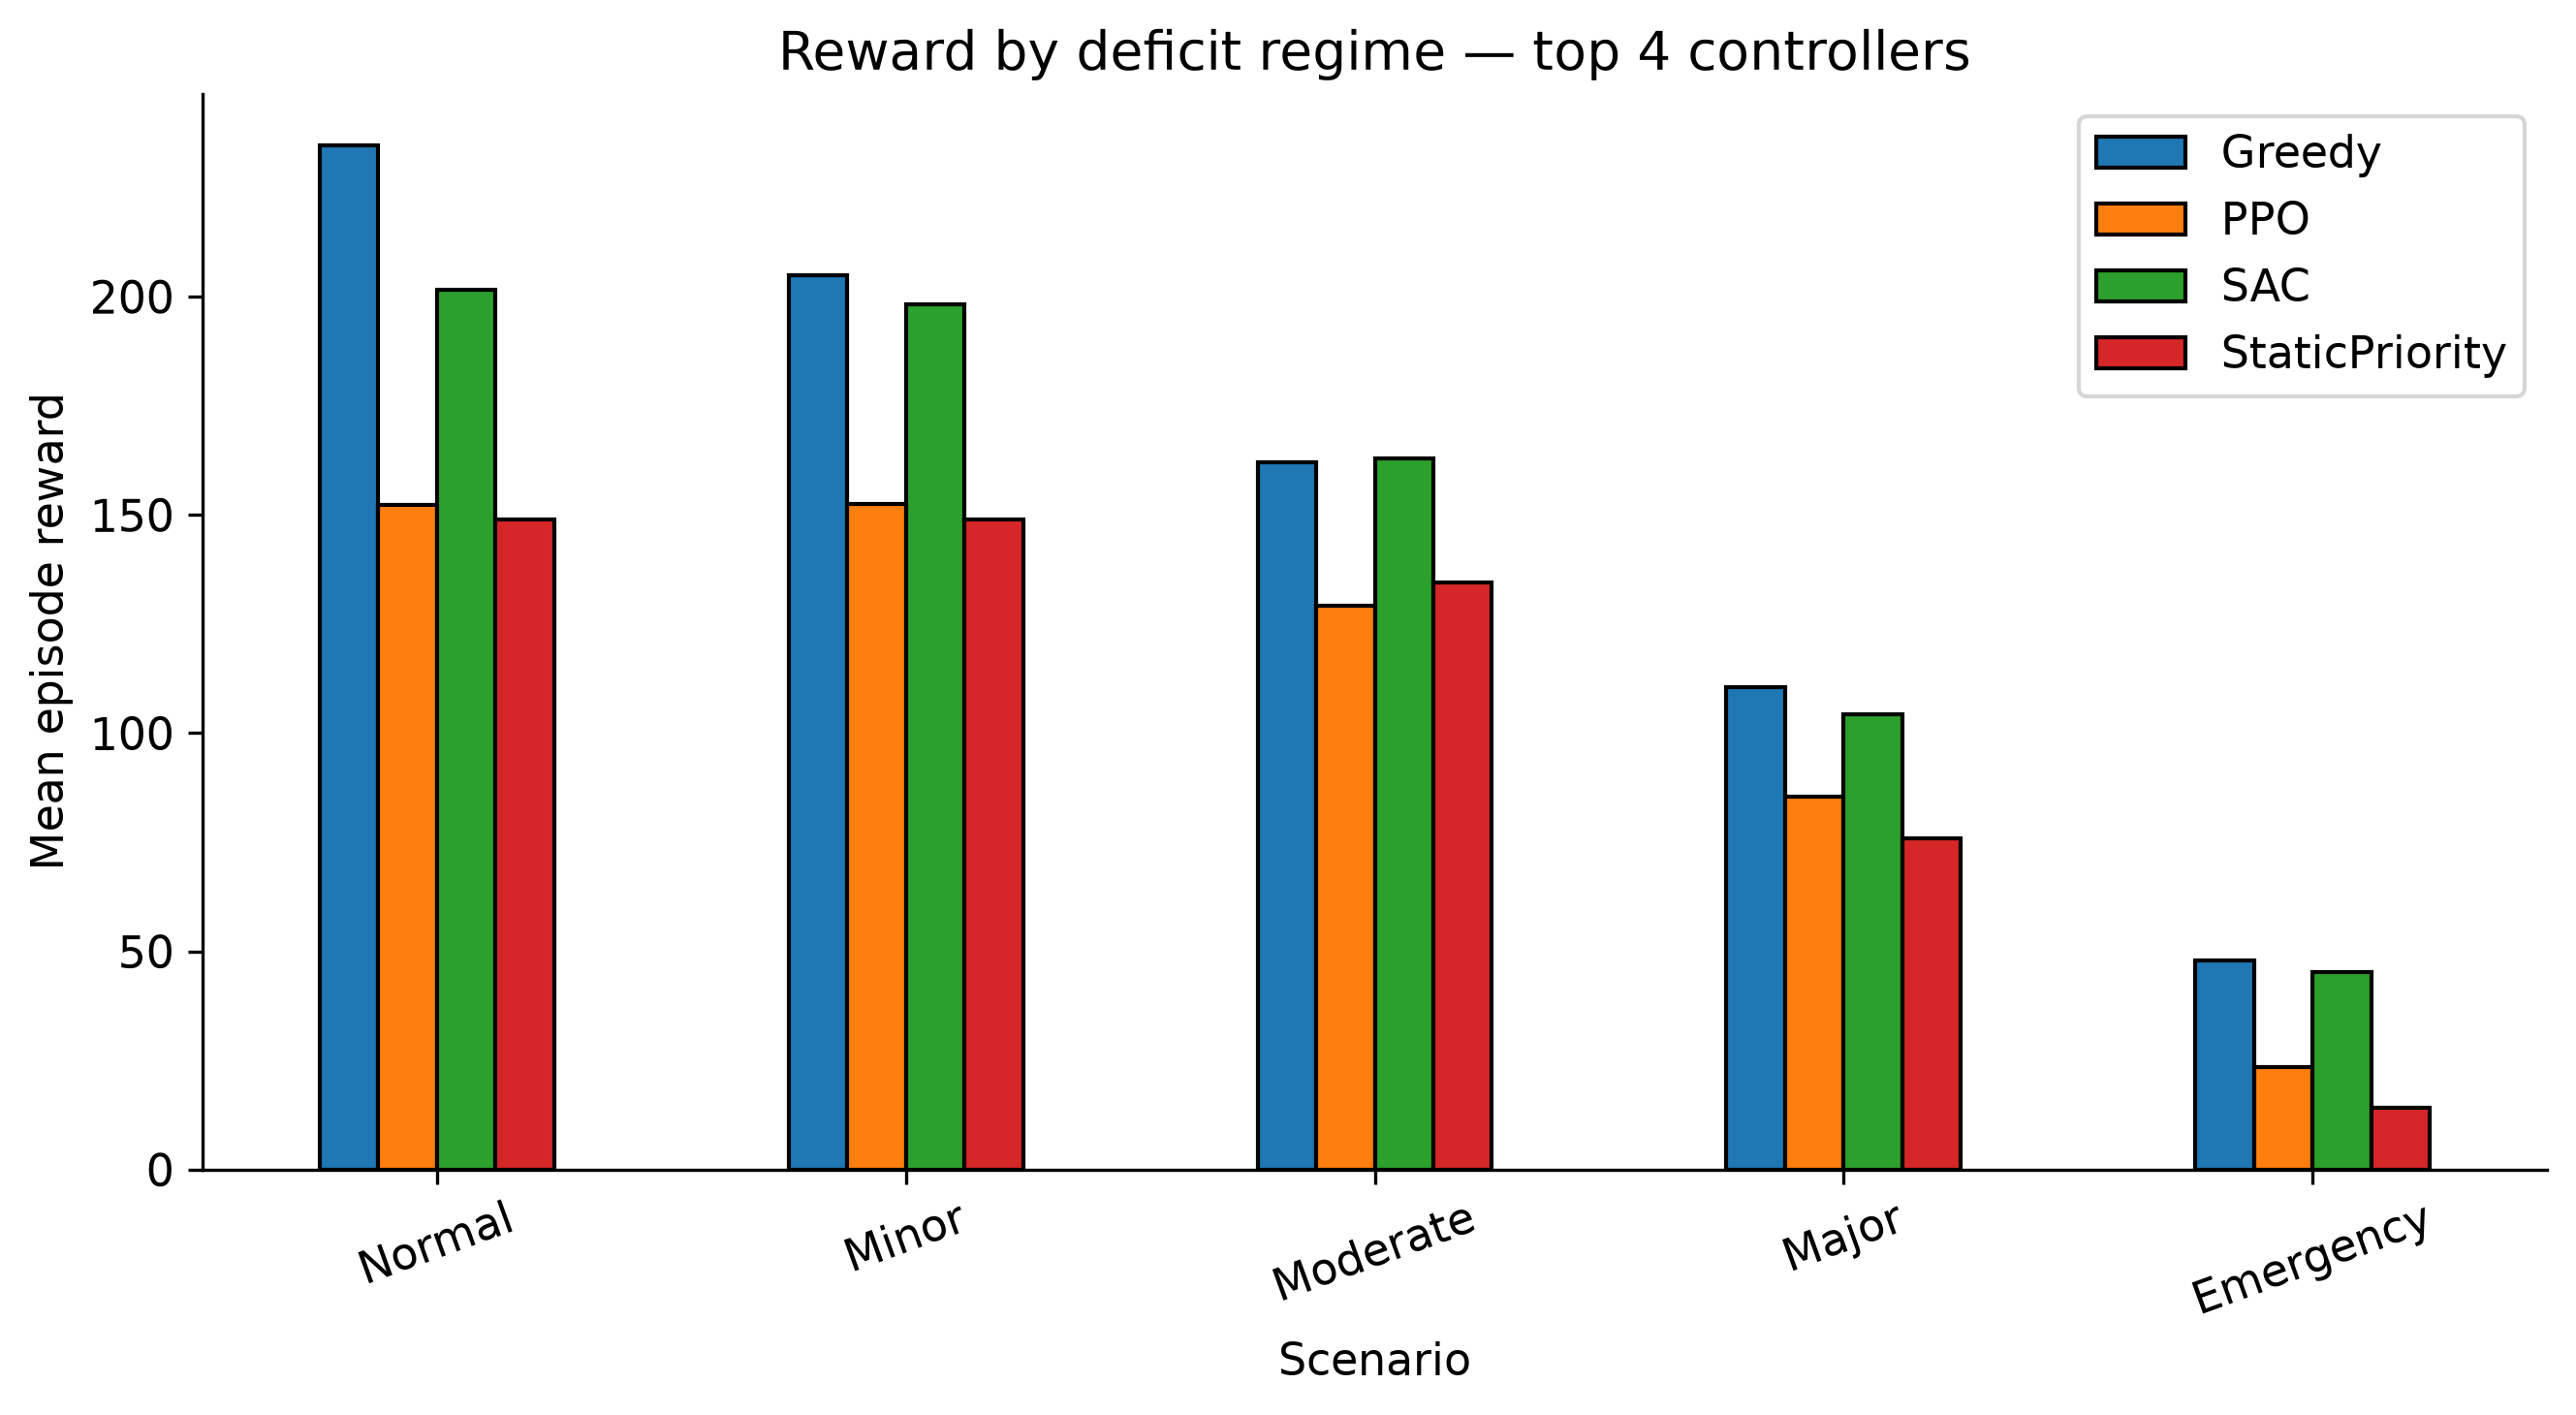
\includegraphics[width=\linewidth]{figures/fig2_regime_reward.png}}
\caption{Per-regime reward for the top four controllers under the corrected protocol. The exact-lookahead Greedy now leads SAC in four of five regimes, including Emergency -- the reverse of the original submission's headline secondary finding.}
\label{fig:regime}
\end{figure}

This reversal is consistent with, and further explained by, the audit in Section~\ref{sec:audit}: the original Greedy's rounding penalty scales with the \emph{size} of the required cut, since a fixed $\pm 0.05$ discretisation error is applied against a larger deficit fraction precisely when the regime is severe. The original paper's claim that "RL's advantage is largest exactly where adaptive control matters most" was therefore, at least in part, an artifact of the baseline being disproportionately weakened by discretisation error under the conditions where curtailment must be largest -- not solely a demonstration of SAC's adaptivity. SAC nonetheless remains highly competitive with the corrected Greedy across all five regimes (within 3--7\% in every regime except Normal, where the gap is 14\%), and continues to substantially outperform the weaker discrete-action PPO and the non-adaptive StaticPriority baseline in every regime, most sharply under Emergency (SAC 45.26 vs.\ StaticPriority 14.06, a 3.2$\times$ margin).

\section{Discussion}
The audit in Section~\ref{sec:audit} shows that the original Random-beats-Greedy anomaly was a property of a specific, fixable implementation detail -- discretisation rounding in the Greedy heuristic -- rather than a fundamental flaw in the reward design; the oversubscription rescale itself is a physically necessary constraint (served power cannot exceed available power), and its interaction with controller behaviour is now reported quantitatively rather than left implicit. Fixing that one detail did more than resolve the anomaly: it also reversed the per-regime finding in Section~\ref{sec:audit} that RL's advantage is largest under Emergency deficit, since the flawed baseline was disproportionately penalised precisely where curtailment needed to be largest.

The corrected results support a more modest, but better-evidenced, set of claims than the original submission. Continuous-action SAC remains highly competitive with the best deterministic heuristics -- within a few reward points of both Lowest-Priority-First and the corrected Greedy in aggregate, and consistently ahead of every discrete-action RL variant -- but it no longer straightforwardly "beats Greedy by 2.6$\times$ under severe deficit," nor is it statistically indistinguishable from the strongest heuristic. Practitioners deploying Reinforcement Learning for campus load shedding should take three points from this: first, cast the curtailment action as a continuous vector rather than discretising, since discrete RL variants uniformly underperform both the continuous-control methods and the strongest heuristics in our benchmark; second, compare against a \emph{correctly implemented} operator-grade baseline before crediting RL with a win, since a plausible-looking heuristic can be silently miscalibrated in a way that specifically inflates RL's apparent advantage under the conditions that matter most; and third, report seed-to-seed variance for any headline claim, since Table~\ref{tab:ranking}'s single-seed ranking of SAC over TD3 reverses when averaged across five seeds.

\emph{Reward-weight sensitivity.} Re-evaluating the trained SAC policy (unchanged network weights) under reward weights $\omega_C \in \{0.5,1,2,4\}$ and $\omega_F \in \{0,0.5,1,2\}$ (Fig.~\ref{fig:weights}) shows reward increasing monotonically in $\omega_F$ and decreasing monotonically in $\omega_C$, as expected given the policy already achieves near-maximal fairness ($J \approx 0.999$) and low critical-cluster curtailment: reweighting a term the policy already satisfies mechanically scales the reward without indicating any hidden trade-off the policy is exploiting. This is consistent with the original notebook's Section-16 analysis and, carried forward here on the corrected agent, does not reveal reward hacking on either axis.

\begin{figure}[tbp]
\centerline{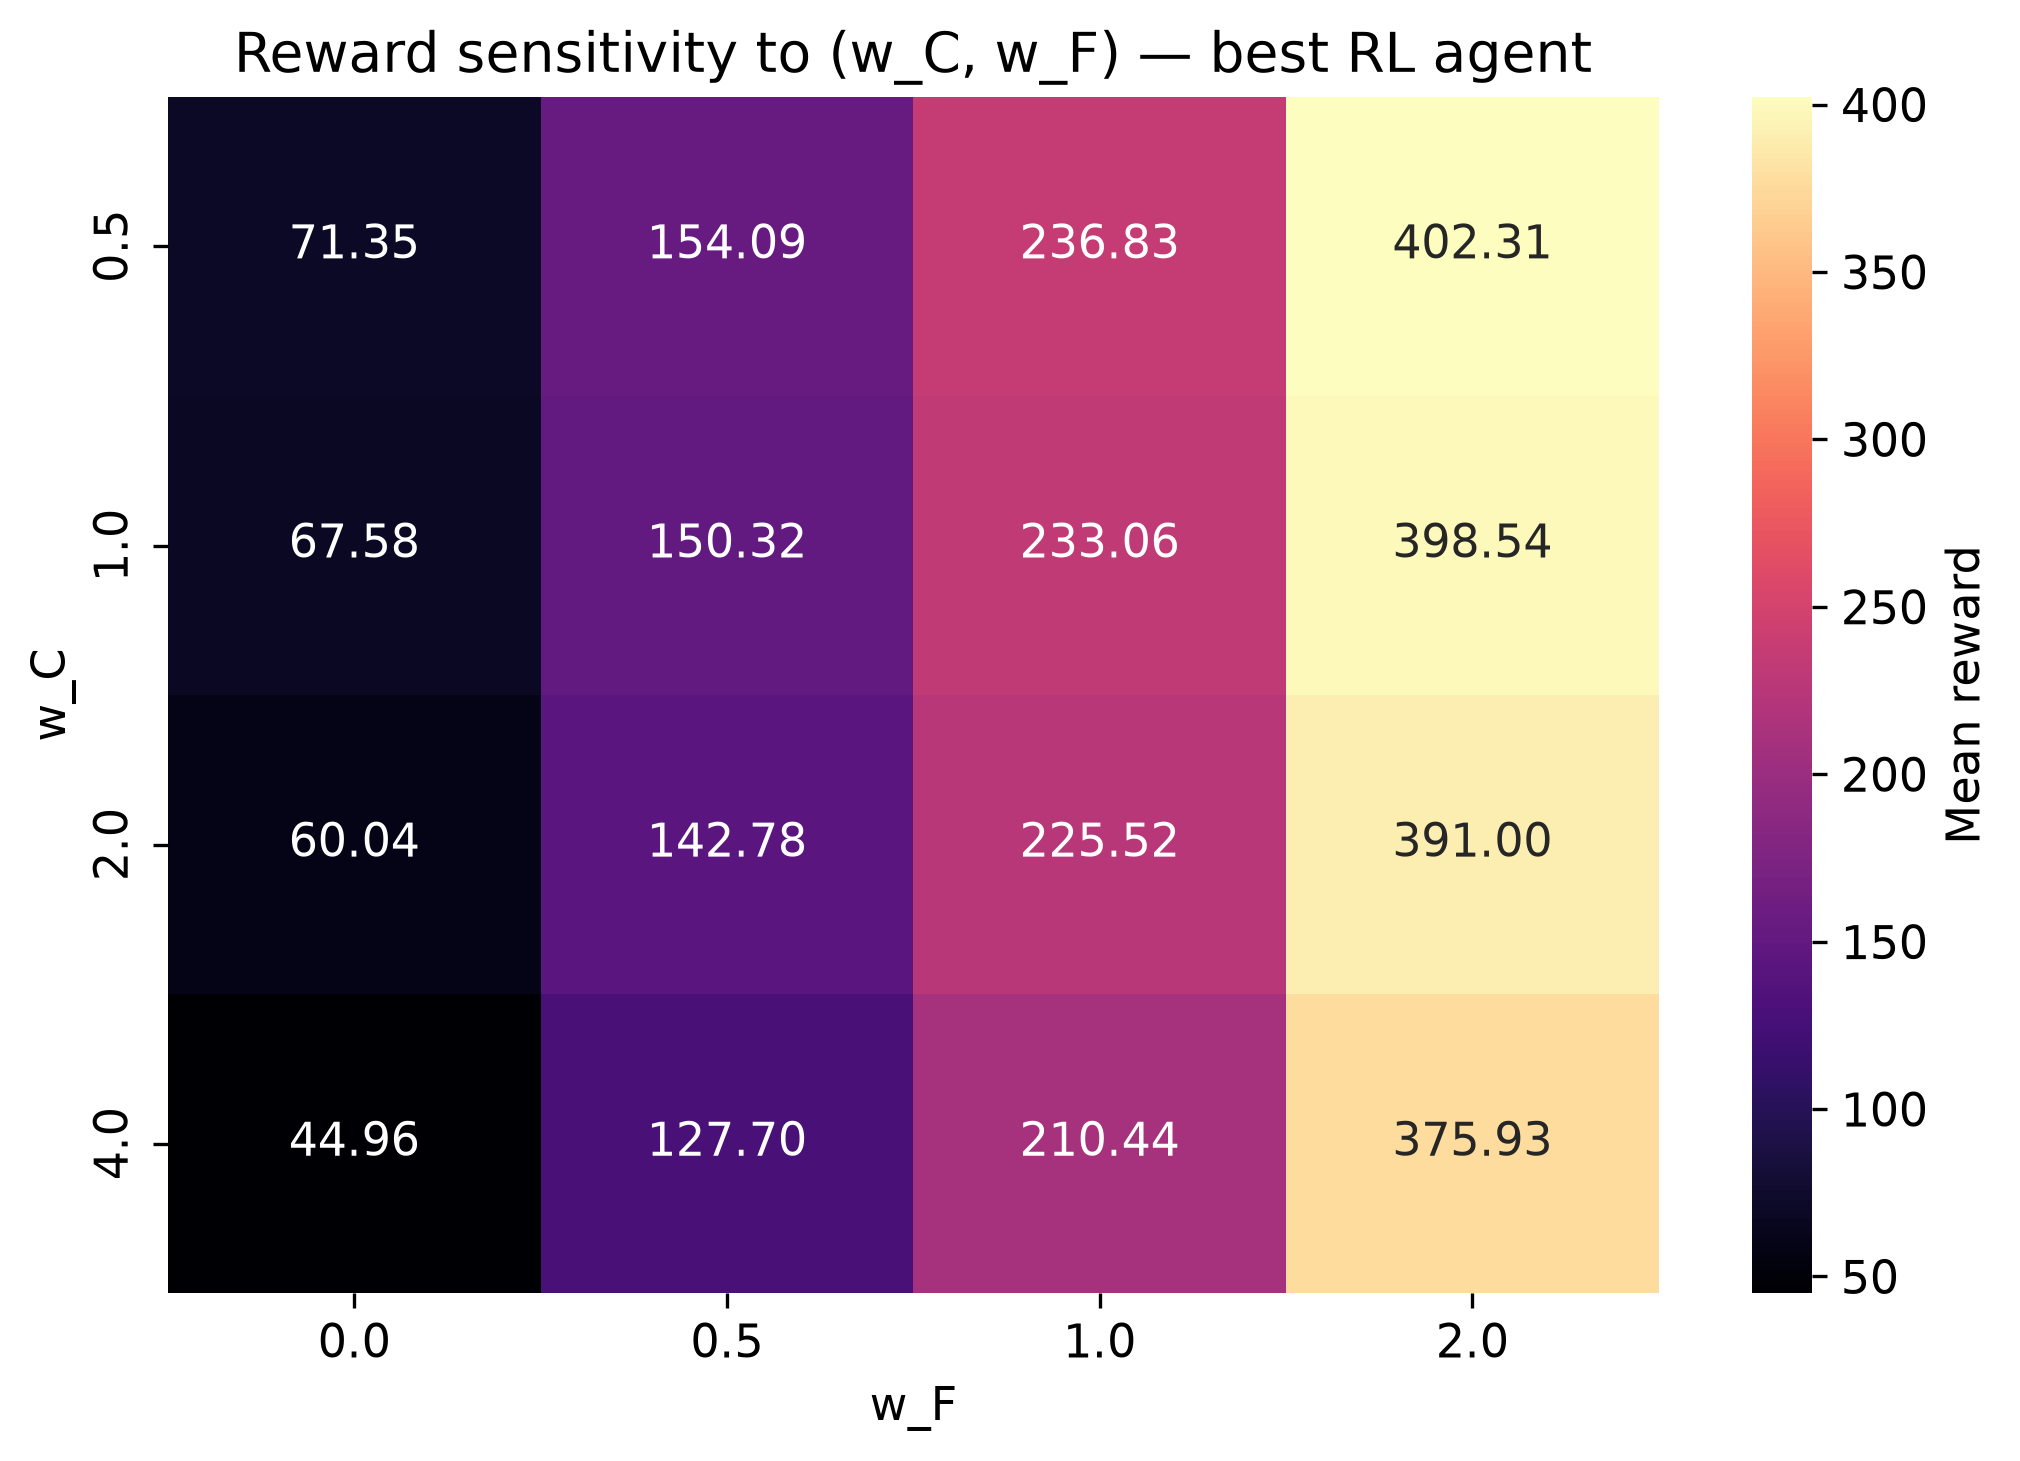
\includegraphics[width=0.85\linewidth]{figures/fig5_weight_heatmap.png}}
\caption{Reward sensitivity of the trained SAC policy to the critical-load weight $\omega_C$ and fairness weight $\omega_F$. Reward scales monotonically with each weight, consistent with a policy that already scores well on both dimensions rather than trading one off against the other.}
\label{fig:weights}
\end{figure}

\emph{Eight feeders vs.\ three clusters.} The 55 buildings are physically wired across eight feeders (Section III-A enumerates them for provenance), but control decisions are made at the coarser three-cluster granularity that the campus Works and Physical Planning Department actually uses operationally for shedding policy; the feeder count is retained in the text solely to describe the physical topology of the dataset, not as a second control granularity.

\section{Conclusion}
We benchmarked fourteen Reinforcement Learning variants against five non-adaptive controllers for load shedding on a five-month dataset from the University of Lagos campus microgrid, under an equalised training budget, multi-seed reporting for the headline controllers, and a Holm-corrected statistical comparison. Continuous-action SAC remains close to the strongest deterministic policy in aggregate reward (141.44 vs.\ Lowest-Priority-First's 143.55) and clearly ahead of every discrete-action RL variant, but the margin over a correctly implemented Greedy controller is +2.54 reward, not the +16.77 originally reported, and averaged across five seeds TD3 (145.0) rather than SAC is the strongest continuous-control method. Action-space representation, not algorithmic family, remains the decisive design choice in this domain: every discrete-action RL variant underperforms both continuous-control methods and the two strongest heuristics, exactly as originally claimed. What the corrected analysis withdraws is the stronger claim that RL decisively beats a well-implemented operator-grade baseline, particularly under severe deficit -- the regime where, once Greedy is fixed, it is RL that must work hardest to keep up.

The immediate research agenda will integrate a noisy multi-step forecast of available power into the state, scale to multi-feeder coordination through multi-agent SAC, and extend the environment with on-site solar generation and battery storage. Returning to the core research question, Reinforcement Learning remains a credible alternative to Greedy on a sub-Saharan campus microgrid provided that the action is treated as continuous, but practitioners should not expect it to dominate a correctly implemented operator-grade baseline by a wide margin: the more defensible case for RL here is competitiveness with strong heuristics under a wide range of conditions, together with the ability to adapt online as campus load patterns or priority tables change, rather than a large fixed performance gap.

\section*{Acknowledgment}

\bibliographystyle{IEEEtran}
\bibliography{references}

\end{document}
